\documentclass[handout]{beamer}
\usetheme{Warsaw}

\usepackage[utf8]{inputenc}
\usepackage[french]{babel}
\usepackage{listings, float, graphicx, amsmath, hyperref}

% Useful tweaks
\setcounter{secnumdepth}{2}
\newcommand{\sectionbreak}{\clearpage}
\hypersetup{
  colorlinks,
  citecolor=blue,
  filecolor=blue,
  linkcolor=blue,
  urlcolor=blue
}

\begin{document}
\title{Exact String Matching Problem}
\subtitle{Recherche de motif}

\author{Grégoire Jadi \and{} Noémi Salaün}
\date{\today}

\frame{\titlepage}

\begin{frame}{The Exact String Matching Problem}
  Un problème vieux comme le monde (de l'informatique):
  \begin{description}
  \item[Brute-Force] 1970
  \item[Morris-Pratt] 1977
  \item[Knuth-Morris-Pratt] 1977
  \end{description}
\end{frame}

\begin{frame}{The Exact String Matching Problem}
  Avec beaucoup d'applications:
  \begin{itemize}
  \item text processing;
  \item image processing;
  \item signal procesing;
  \item \texttt{<insert your favorite field here>} processing.
  \end{itemize}
\end{frame}

\begin{frame}{The Exact String Matching Problem}
  Différentes classes d'algorithmes pour différents types de problèmes:
  \begin{itemize}
  \item basé sur la comparaison de caractère uniquement;
  \item basé sur un automate;
  \item basé sur la parallélisation de bits (\emph{bits parallelism}).
  \end{itemize}
\end{frame}

\begin{frame}{\texttt{SA}\^{}W \texttt{BMH}}
  L'algorithme \emph{Shift-And} err, no, \emph{Boyer-Moore-Horspool} est un algorithme:
  \begin{itemize}
  \item dérivé de \emph{Boyer-Moore} lui même dérivé de \emph{Knut-Morris-Pratt};
  \item basé sur la comparaison de caractère uniquement.
  \end{itemize}
\end{frame}

\begin{frame}{\texttt{BMH}}
  Recherche de motifs de taille: 2, 4, 8, 16, 32, 64, 128, 256:
  
  \begin{tabular}{|l|c|c|c|c|c|c|c|c|c|}
    \hline
    Fichier             & $ | \Sigma | $ & ~Temps \\
    \hline

    bible.txt (3.9M)    & 63 & 4.2s \\    
    E.coli (4.5M)       & 4  & 1.3s \\
    world192.txt (2.4M) & 94 & 3.4s \\
    hi (504K)           & 20 & 0.2s \\
    hs (3.2M)           & 19 & 1.7s \\
    mj (444K)           & 20 & 0.2s \\
    sc (2.8M)           & 20 & 1.4s \\
    \hline

  \end{tabular}
\end{frame}

\begin{frame}{\texttt{EBOM}}
  L'algorithme \texttt{EBOM} ou \emph{Extended BOM} ou \emph{Extended Backward-Oracle-Matching} est un algorithme:
  \begin{itemize}
  \item dérivé de \texttt{BOM} lui même dérivé de \texttt{BDM};
  \item basé sur un automate.
  \end{itemize}
\end{frame}

\begin{frame}{\texttt{BDM}\^{}W Yo \texttt{DAWG}}
  \begin{figure}[h]
    \centering
    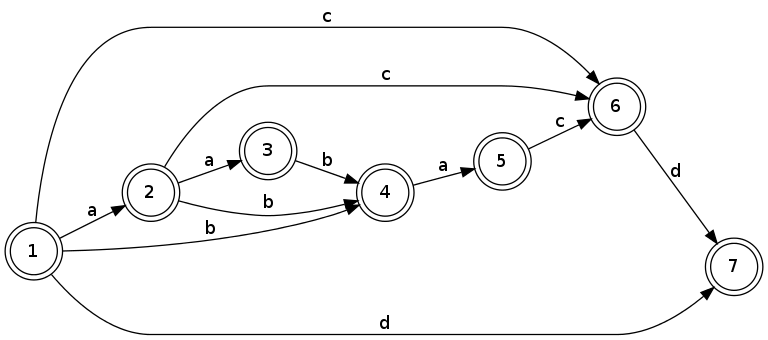
\includegraphics[width=10cm]{dawg.png}
    \caption{DAWG de "aabacd"}
    \label{fig:dawg}
  \end{figure}
\end{frame}

\begin{frame}{Conclusion}
  \begin{itemize}
  \item fun;
  \item énervant;
  \item long;
  \item intéressant.
  \end{itemize}
\end{frame}


\end{document}
